\documentclass[12pt,a4paper]{article}
\usepackage{algorithm, algpseudocode, amsmath, amssymb, amsthm, bm, csquotes, emf, empheq, geometry, graphicx, hyperref, listings, mhchem, multirow, siunitx, slashbox, subcaption, upgreek}
\usepackage[italicdiff]{physics}
\usepackage[section]{placeins}
\usepackage[justification=centering]{caption}
\usepackage[column=O]{cellspace}
\usepackage[extrafootnotefeatures]{xepersian}
\hypersetup{colorlinks=true, urlcolor=cyan}

\title{تمرین سری دوم دینامیک غیرخطی و آشوب}
\author{صالح شاملو احمدی\\شماره دانشجویی: ۹۸۱۰۰۸۷۲}
\date{۲۷ بهمن ۱۴۰۱}

\settextfont{Yas}

\setlength\cellspacetoplimit{4pt}
\setlength\cellspacebottomlimit{3pt}
\newcommand{\multlinecell}[1]{\begin{tabular}[c]{@{}c@{}}#1\end{tabular}}

\newcommand\qfrac[2]{\left(\frac{#1}{#2}\right)}
\newcommand\fsqrt[2]{\sqrt{\frac{#1}{#2}}}
\newcommand\ddfrac[2]{{\displaystyle\frac{\displaystyle #1}{\displaystyle #2}}}
\newcommand\pdvc[3]{\qfrac{\partial #1}{\partial #2}_{#3}}
\newcommand{\dbar}{{d\mkern-7mu\mathchar'26\mkern-2mu}}
\newcommand*{\defeq}{\mathrel{\vcenter{\baselineskip0.5ex \lineskiplimit0pt
			\hbox{\scriptsize.}\hbox{\scriptsize.}}}
	=}

\begin{document}
	\maketitle
	\section*{\lr{2.5.6}}
	\subsection*{\lr{(a)}}
	طبق قانون پیوستگی (که از بقای جرم می‌آید)، در جایی که چگالی ثابت است، میزان سیال ورودی باید با میزان سیال خروجی برابر باشد.
	در واحد زمان، این همان رابطه
	\begin{equation}
		av(t) = A\dot{h}(t) \label{p1:cont}
	\end{equation}
	است (سرعت آب ورودی با سرعت پایین آمدن سطح آب برابر است).
	\subsection*{\lr{(b)}}
	طبق بقای جرم، جرم آبی که از سطل کم می‌شود با جرم آبی که به آب خروجی اضافه می‌شود برابر است. پس، طبق بقای انرژی،
	\begin{align}
		\Delta{U}_{\text{آب داخل سطل}} &= \Delta{K}_{\text{آب خروجی}}, \\
		\Delta{m}gh &= \frac{\Delta{m} v^2}{2}, \\
		v^2 &= 2gh. \label{p1:energy}
	\end{align}
	\subsection*{\lr{(c)}}
	با جایگذاری $v$ از \eqref{p1:cont} داخل \eqref{p1:energy}
	\begin{gather}
		\qfrac{A\dot(h)}{a}^2 = 2gh \implies \\
		\dot{h} = \sqrt{2gh}\qfrac{a}{A}
	\end{gather}
	\subsection*{\lr{(d)}}
	معادله را برای $t < 0 $ حل می‌کنیم:
	\begin{align}
		\int_{h(t)}^{0}\frac{\dd{h}}{h} &= \sqrt{2g}\qfrac{a}{A}\int_{t}^{0}\dd{t} \\
		-2\sqrt{h(t)} &= -\sqrt{2g}\qfrac{a}{A}t \\
		h(t) &= \frac{gt^2}{2}\qfrac{a}{A}^2
	\end{align}
	از این جواب به نظر می‌رسد پاسخ یکتا است، اما چیزی که در نظر نگرفتیم این است که اگر ظرف خالی شده باشد، $\dot{h}$ برابر صفر است
	و دیگر انتگرال بالا معنی نمی‌دهد. در این حالت نمودار $h(t)$ ابتدا یک سهمی مانند رابطه‌ای است که بدست آوردیم و هنگامی که $h(t)$
	به صفر می‌رسد، روی $h = 0 $ باقی می‌ماند. این نقطه می‌تواند هر جایی در بازه $t\le0 $ باشد، پس جواب معادله یکتا نیست.
	\section*{\lr{2.8.3}}
	\subsection*{\lr{(a)}}
	\begin{gather}
		\int_{x(0)}^{x(t)}\frac{\dd{x}}{x} = -\int_{0}^{t}t \\
		\ln(\frac{x(t)}{x(0)}) = -t \\
		\boxed{x(t) = x(0)e^{-t}} = e^{-t}
	\end{gather}
	\begin{equation}
		x(1) = \frac{1}{e} \approx 0.36787944117144233
	\end{equation}
	\subsection*{\lr{(b)}}
	\begin{empheq}[left=\empheqlbrace]{align}
		\Delta{t} = 1&: \hat{x}(1) = 0.0 \\
		\Delta{t} = 10^{-1}&: \hat{x}(1) = 0.3486784401 \\
		\Delta{t} = 10^{-2}&: \hat{x}(1) = 0.3660323412732296 \\
		\Delta{t} = 10^{-3}&: \hat{x}(1) = 0.36769542477096373 \\
		\Delta{t} = 10^{-4}&: \hat{x}(1) = 0.36786104643292905 \\
	\end{empheq}
	\subsection*{\lr{(c)}}
	\begin{figure}[h!]
		\centering
		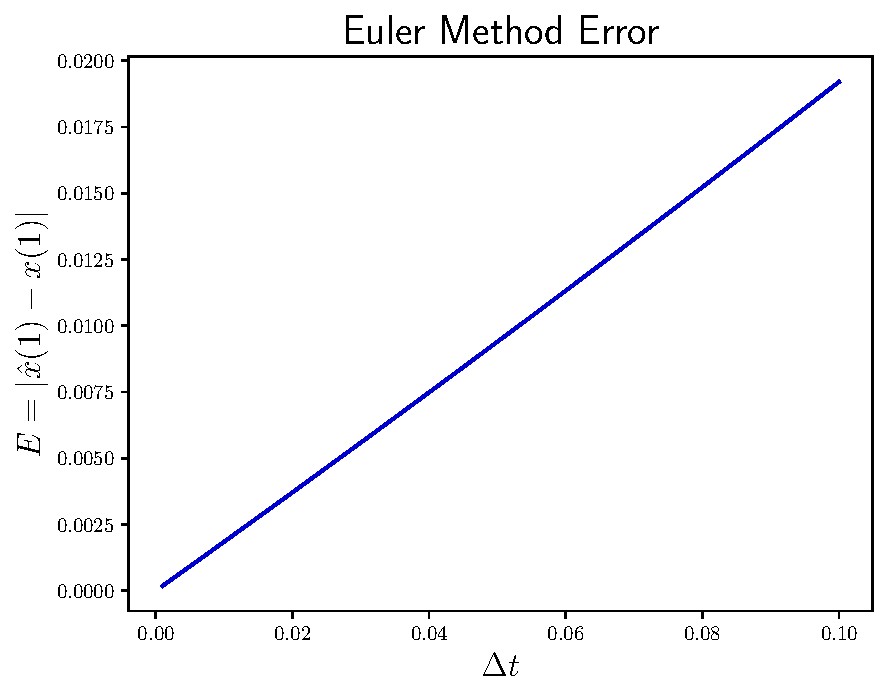
\includegraphics[width=0.65\linewidth]{fig/euler-error}
		\caption{خطای مقدار $x(1)$ برحسب $\Delta{t}$ در روش اویلر. از همین نمودار مشخص است که خطای روش اویلر، خطی است.}
	\end{figure}
	\begin{figure}[h!]
		\centering
		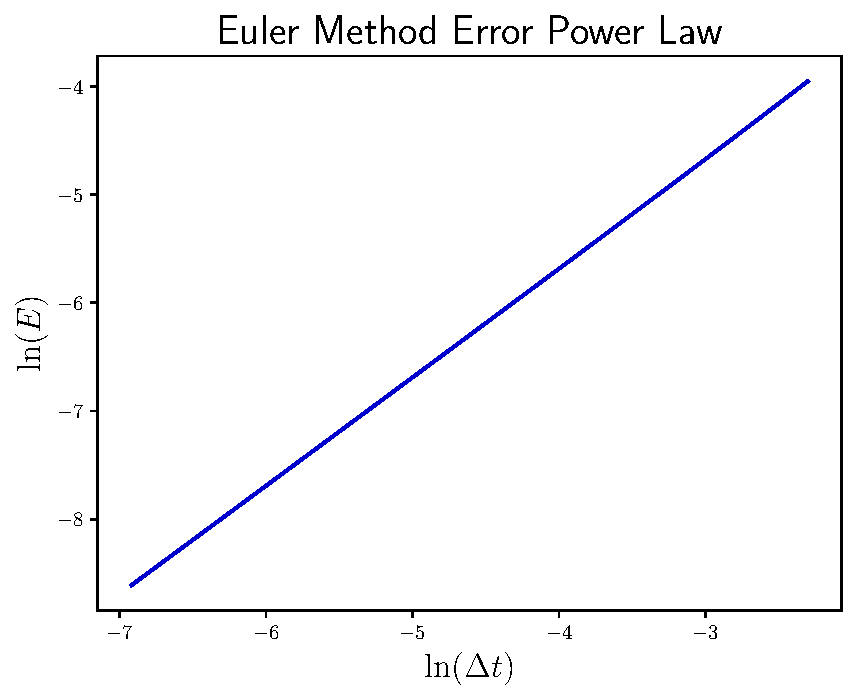
\includegraphics[width=0.65\linewidth]{fig/euler-error-loglog}
		\caption{نمودار تمام لوگاریتمی خطای مقدار $x(1)$ برحسب $\Delta{t}$ در روش اویلر.
			از شیب این نمودار نیز نتیجه می‌گیریم خطای روش اویلر، خطی است (شیب این نمودار برابر یک است).}
	\end{figure}
	\section*{\lr{2.8.5}}
	\begin{empheq}[left=\empheqlbrace]{align}
		\Delta{t} = 1&: \hat{x}(1) = 0.375 \\
		\Delta{t} = 10^{-1}&: \hat{x}(1) = 0.3678797744124984 \\
		\Delta{t} = 10^{-2}&: \hat{x}(1) = 0.3678794412023554 \\
		\Delta{t} = 10^{-3}&: \hat{x}(1) = 0.36787944117144633 \\
		\Delta{t} = 10^{-4}&: \hat{x}(1) = 0.367879441171445 \\
	\end{empheq}
	\begin{figure}[h!]
		\centering
		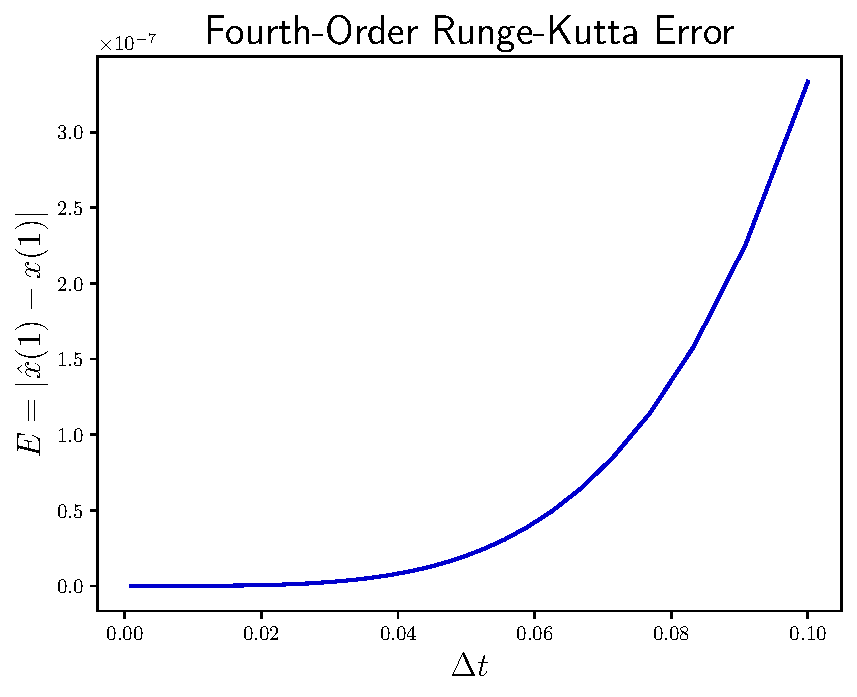
\includegraphics[width=\linewidth]{fig/rk4-error}
		\caption{خطای مقدار $x(1)$ برحسب $\Delta{t}$ در روش رونگه--کوتا مرتبه چهارم.}
	\end{figure}
	\begin{figure}[h!]
		\centering
		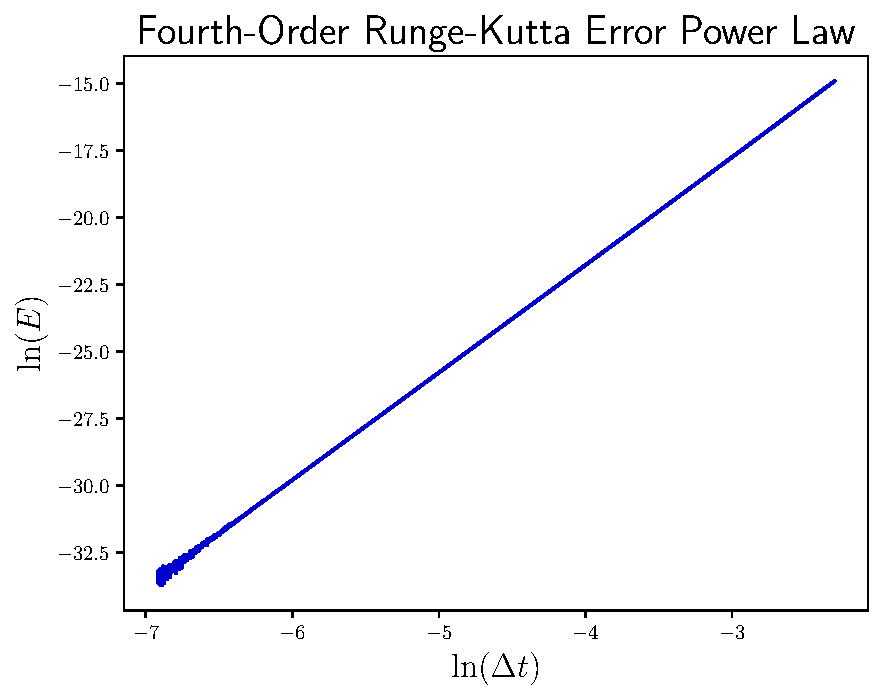
\includegraphics[width=\linewidth]{fig/rk4-error-loglog}
		\caption{نمودار تمام لوگاریتمی خطای مقدار $x(1)$ برحسب $\Delta{t}$ در روش رونگه--کوتا مرتبه چهارم.
			شیب این نمودار برابر $4$ است، پس خطای روش رونگه--کوتا مرتبه چهارم، از مرتبه چهارم $\Delta{t}$ است.}
	\end{figure}
	\section*{\lr{2.8.9}}
	\begin{empheq}[left={\text{معادلات روش رونگه--کوتا مرتبه چهارم}\empheqlbrace}]{align}
		k_1 &= f(x_n) \\
		k_2 &= f\qty(x_n + \frac{1}{2}k_1\Delta t) \\
		k_3 &= f\qty(x_n + \frac{1}{2}k_2\Delta t) \\
		k_4 &= f(x_n + k_3\Delta t) \\
		x_{n+1} &= x_n + \frac{1}{6}(k_1 + 2k_2 + 2k_3 + k_4)\Delta t
	\end{empheq}
	با بسط اویلر حول نقطه $t$، اختلاف  روش رونگه--کوتا مرتبه چهارم را با مقدار اصلی حساب می‌کنیم:
	\begin{multline}
		x_{n+1} - x(t+\Delta{t}) = x_n + \frac{1}{6}(k_1 + 2k_2 + 2k_3 + k_4)\Delta t -\left(x + \dv{x}{t}\Delta t\right. \\
		\left. + \frac{1}{2!}\dv[2]{x}{t}\Delta t^2 + \frac{1}{3!}\dv[3]{x}{t}\Delta t^3 + \frac{1}{4!}\dv[4]{x}{t}\Delta t^4
		+ \frac{1}{5!}\dv[5]{x}{t}\Delta t^5 + \mathcal{O}(\Delta t^6)\right)
	\end{multline}
	برای محاسبه خطای موضعی، $x_n = x(t)$. در رابطه بالا با استفاده از قاعده زنجیری، می‌توانیم مشتق‌های $x$
	نسبت به t را با مشتق‌های $f$ نسبت به $x$ جایگزین کنیم. بدین شکل که
	\begin{equation}
		\dv{x}{t} = f(x) \implies \dv[2]{x}{t} = \dv{f}{t} = \dv{f}{x}\dv{x}{t} = f(x)\dv{f}{x}
	\end{equation}
	و مشابه همین برای بقیه مشتق‌ها. به‌طور کلی تبدیل
	\begin{equation}
		\dv{t} \rightarrow \dv{x}{t}\dv{x} = f(x)\dv{x}
	\end{equation}
	مشتق‌های $t$ را با مشتق‌های $x$ جایگزین می‌کند. دلیل این تبدیل، این است که بتوانیم بسط تیلور $k$ها را با بسط تیلور $x(t+\Delta{t})$
	مقایسه کنیم. با جایگذاری $k$ها یکی پس از دیگری و بسط تیلور، همه رابطه را برحسب $f$ و مشتقات آن نسبت به $x$ بازنویسی می‌کنیم
	و مرتبه خطا را برحسب $\Delta t$ بدست می‌آوریم.
	\begin{multline}
		x_{n+1} - x(t+\Delta{t}) = \frac{1}{6}(k_1 + 2k_2 + 2k_3 + k_4)\Delta t - f(x)\Delta t \left(1 + \frac{\Delta t}{2} \dv{f}{x} \right. \\
		+ \frac{\Delta t^2}{6} \qty[\qty(\dv{f}{x})^2 + f(x) \dv[2]{f}{x}] + \frac{\Delta t^3}{24}
		\qty[f^2(x) \dv[3]{f}{x} + \dv{f}{x}\qty(\dv{f}{x} + 4 f(x) \dv[2]{f}{x})] \\
		+ \frac{\Delta t^4}{120} \left[4 f^2(x) \qty(\dv[2]{f}{x})^2 + \qty(\dv{f}{x})^4 + 7 f^2(x) \dv[3]{f}{x} \dv{f}{x}
		+ f^3(x) \dv[4]{f}{x} \right. \\
		\left.\left.+ 11 f(x) \qty(\dv{f}{x})^2 \dv[2]{f}{x}\right] + \mathcal{O}(\Delta t^5)\right)
	\end{multline}
	\begin{equation}
		k_1 = f(x)
	\end{equation}
	\begin{multline}
		k_2 = f(x)\left[1 + \frac{1}{2} \Delta t \dv{f}{x} + \frac{1}{8} \Delta t^2 \dv[2]{f}{x}f(x)
		+ \frac{1}{48} \Delta t^3 \dv[3]{f}{x} f(x)^2\right. \\
		\left. + \frac{1}{384} \Delta t^4 \dv[4]{f}{x} f(x)^3 + \mathcal{O}(\Delta t^5)\right]
	\end{multline}
	\begin{multline}
		k_3 = \left[\mathcal{O}(\Delta t^5) + \frac{1}{384} \Delta t^4 f^4(x) \dv[4]{f}{x}+\frac{1}{48} \Delta t^3 f^3(x) \dv[3]{f}{x}
		+\frac{1}{32} \Delta t^4 f^3(x) \qty(\dv[2]{f}{x})^2 \right. \\
		+\frac{1}{8} \Delta t^2 f^2(x) \dv[2]{f}{x}+\frac{1}{4} \Delta t^2 f(x) \qty(\dv{f}{x})^2+\frac{1}{2} \Delta t f(x) \dv{f}{x}
		+\frac{1}{24} \Delta t^4 f^3(x) \dv[3]{f}{x} \dv{f}{x} \\
		\left.+\frac{1}{32} \Delta t^4 f^2(x) \qty(\dv{f}{x})^2 \dv[2]{f}{x}
		+\frac{3}{16} \Delta t^3 f^2(x) \dv{f}{x} \dv[2]{f}{x}+f(x)\right]
	\end{multline}
	\begin{multline}
		k_4 = \left[\mathcal{O}(\Delta t^5) + \frac{1}{6} \Delta t^3 f^3(x) \dv[3]{f}{x}+\frac{1}{8} \Delta t^4 f^3(x) \qty(\dv[2]{f}{x})^2
		+\frac{1}{2} \Delta t^2 f^2(x) \dv[2]{f}{x} \right. \\
		+\frac{1}{4} \Delta t^3 f(x) \qty(\dv{f}{x})^3+\frac{1}{2} \Delta t^2 f(x) \qty(\dv{f}{x})^2 + \Delta t f(x) \dv{f}{x}
		+\frac{13}{48}\Delta t^4 f^3(x) \dv[3]{f}{x} \dv{f}{x} \\
		\left. +\frac{9}{16} \Delta t^4 f^2(x) \qty(\dv{f}{x})^2 \dv[2]{f}{x}
		+\frac{5}{8} \Delta t^3 f^2(x) \dv{f}{x} \dv[2]{f}{x}+f(x)\right]
	\end{multline}
	\begin{multline}
		x_{n+1} - x(t+\Delta{t}) = \Delta t^5\left[-\frac{19}{2880} f^4(x) \dv[4]{f}{x}(x)-\frac{1}{480} f^3(x) \qty(\dv[2]{f}{x})^2
		-\frac{1}{120} f(x) \dv{f}{x}^4 \right. \\
		\left.+\frac{1}{1440}f^3(x)\dv{f}{x}\dv[3]{f}{x}(x)+\frac{1}{80} f^2(x) \qty(\dv{f}{x})^2 \dv[2]{f}{x}\right] + \mathcal{O}(\Delta t^6)
	\end{multline}
	بنابراین خطای موضعی روش رونگه--کوتا مرتبه چهارم از مرتبه پنجم $\Delta t$ است.
\end{document}